\ifdefined\MAINDOC\else
\documentclass[10pt, a4paper, fleqn]{article}
\usepackage{base}

\begin{document}
    \title{Skript Mathe 2}
    \date{11. Juni 2018}
    \maketitle
\fi

Erhalte Intervallschachtelung $[a_n, b_n]$ mit
\begin{itemize}
    \item $a_n \nearrow, b_n \searrow$
    \item $b_n - a_n \to 0$
    \item $a_n \leq b_n$
\end{itemize}
\[
    \underset{1.26}{\imp} \lim_{n \to \infty} a_n = \lim_{n \to \infty} b_n = c
\]

Es ist $f(a_n) \leq 0, f(b_n) \geq 0 \ \forall n \in \IN$.
Da $f$ stetig, gilt:
\[\begin{aligned}
    & \underbrace{\lim_{n \to \infty} f(a_n)}_{\leq 0} = f(c) \\
    & \underbrace{\lim_{n \to \infty} f(b_n)}_{\geq 0} = f(c) \\
    & \imp f(c) = 0 \qed
\end{aligned}\]

Dieses Verfahren verwendet man auch zur Nullstellenberechnung.

\subsection{Satz: Zwischenwertsatz allgemein}
$f: [a, b] \to \IR$ stetig, $y$ sei eine Zahl zwischen $f(a)$ und $f(b)$.

Dann gibt es $\overline{x} \in [a, b]$ mit $f(\overline{x}) = y$.

\textbf{Beweis: }

Ohne Beschränkung der Allgemeinheit (o.B.d.A)
\[
    f(a) \geq y \geq f(b)    
\]
Setze $g: [a, b] \to \IR, x \to f(x) - y \imp$
\begin{itemize}
    \item $g(a) = f(a) - y \geq 0$
    \item $g(b) = f(b) - y \geq 0$
    \item $g$ stetig
\end{itemize}
\[
    \imp \exists \ \overline{x} \in [a, b]: y(\overline{x}) = 0 \imp f(\overline{x}) = g \qed    
\]

\subsection{Satz}
Sei $D$ ein Intevall, $f: D \to \IR$ stetig. Dann gilt:
\begin{enumerate}[1.]
    \item $f(D)$ Intervall oder enthält genau ein Element
    \item $f$ injektiv $\eqv$ $f$ streng monoton
\end{enumerate}
\textbf{Beweis: }

\begin{enumerate}
    \item Falls $f(D)$ nur ein Element enthält: fertig \checkmark

    Enthalte $f(D)$ mindestens 2 Elemente $y_1 < y_2.$
    \[\begin{aligned}
        &\imp \exists x_1, x_2 \in D: & f(x_1) = y_1 \\
        &&f(x_2) = y_2 \\
        &\imp x_1 \neq x_2
    \end{aligned}\]
    Zeige: Jedes $y \in [y_1, y_2]$ ist in $f(D)$:

    Falls $x_1 < x_2$, gibt es wegen 5.24 ein $x \in \underbrace{[x_1, x_2]}_{\subseteq D}$ 
    mit $f(x) = y$. \\
    Analog für $x_2 < x_1$.
    \[
        \imp y \in f(D) \imp f(D) \text{ Intervall.}    
    \]

    \item $(\Leftarrow)$: Hierzu braucht man die Stetigkeit nicht:

    $f$ streng monoton wachsend (fallend). Sei $x = y$. \\
    O.B.d.A: $x < y$
    \[
        \imp f(x) \underset{\hbox{(>)}}{<} f(y) \imp f(x) \neq f(y)    
    \]
    $(\Rightarrow)$: Hierzu braucht man die Stetigkeit: 
    
    Kontraposition: Sei $f$ nicht
    streng monoton.
    \[\begin{aligned}
        &\imp \exists x < y < z \in D: f(x) < f(y) \text{ und } f(y) \geq f(z) \\ 
        &(\text{oder } f(x) \geq f(y) \text{ und } f(y) \leq f(z)).
    \end{aligned}\]
    $\underset{5.24}{\imp}$ \begin{itemize}
        \item $f$ nimmt in $[x, y]$ jeden Wert zwischen $f(x)$ und $f(y)$ an.
        \item $f$ nimmt in $[y, z]$ jeden Wert zwischen $f(y)$ und $f(z)$ an.
    \end{itemize}
    $\imp$ Mindestens ein Wert wird doppelt getroffen. $\qed$
\end{enumerate}

\subsection{Satz}
Sei $D \subseteq \IR$ Intervall und $f: D \to f(D)$ bijektiv und stetig.

Dann gilt für die Umkehrfunktion $f^{-1}$
\begin{enumerate}[1.]
    \item $f^{-1}$ ist im selben Sinne streng monoton wie $f$
    \item $f^{-1}$ ist stetig
\end{enumerate}

\textbf{Beweis: }
\begin{enumerate}[1.]
    \item $f$ stetig und injektiv $\underset{5.25/2.}{\imp} f$ streng monoton. \\
    Zeige Aussage für $f$ streng monoton wachsend:

    Für $y_1 < y_2; \ y_1, y_2 \in f(D)$ gibt es $x_1 \neq x_2$ mit \\
    $f(x_1) = y_1, f(x_2) = y_2$.

    %TODO Underset
    Es gilt: $\underbrace{y_1}_{= f(x_1)} < \underbrace{y_2}_{= f(x_2)} 
    \underset{\substack{f \text{ streng monoton} \\ \text{ wachsend}}}{\eqv} x_1 < x_2$

    \[\begin{aligned}
        &\eqv f^{-1}(y_1) < f^{-1}(y_2) \\
        &\imp f^{-1} \text{ streng monoton wachsend}
    \end{aligned}\]

    \item $f$ stetig und injektiv $\underset{5.25}{\imp} f(D)$ Intervall, 
    $f$ streng monoton.
\end{enumerate}

\textbf{Annahme: } $f$ streng monoton waschend.

Sei $y_0 \in f(D)$. z.Z: $f^{-1}$ stetig in $y_0$.
Setze $x_0 := f^{-1}(y_0)$.

1. Fall: $x_0$ kein Randpunkt von $D$. 

Mit $\epsilon$--$\delta$--Kriterium:
Sei $\epsilon > 0$, so dass $(x_0 - \epsilon, x_0 + \epsilon) \subseteq D$.

$f$ streng monoton wachsend
\[\begin{aligned}
    &\imp f(x_0 - \epsilon) < y_0 < f(x_0 + \epsilon) \\
    &\imp (f(x_0 - \epsilon), f(x_0 + \epsilon)) \subseteq f(D)
\end{aligned}\]
da $f(D)$ Intevall.

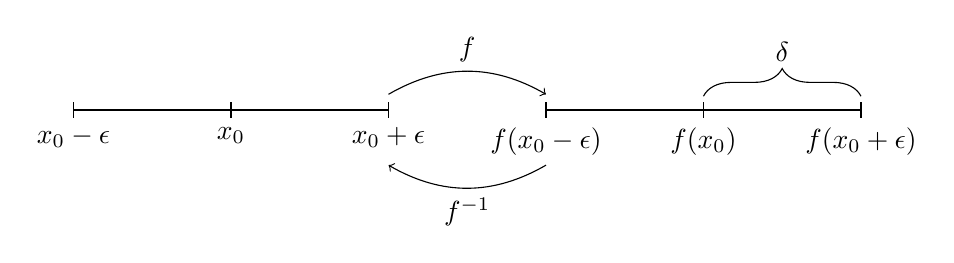
\begin{tikzpicture}
    \draw (0, 0) -- (4, 0);
    \draw (6, 0) -- (10, 0);

    \foreach \x/\xtext in {
        0/$x_0 - \epsilon$, 2/$x_0$, 4/$x_0 + \epsilon$,
        6/$f(x_0 - \epsilon)$, 8/$f(x_0)$, 10/$f(x_0 + \epsilon)$}
        \draw (\x, 0.1) -- (\x, -0.1) node[below] {\xtext};

    \draw[decorate, decoration = {brace, amplitude = 10pt, raise = 5pt}] (8, 0) -- node[above = 14pt] {$\delta$} (10, 0);

    \draw[->] (4, 0.2) to[out = 30, in = 150] node[midway, above] {$f$} (6, 0.2);
    \draw[->] (6, -0.7) to[out = -150, in = -30] node[midway, below] {$f^{-1}$} (4, -0.7);
\end{tikzpicture}

Sei $\delta := \min\{|y_0 - f(x_0 + \delta)|, |y_0 - f(x_0 - \epsilon)|\}$

$\imp f^{-1}((y_0 - \delta, y_0 + \delta)) \subseteq (x_0 - \epsilon, x_0 + \epsilon)$

D.h.: $|y-y_0| < \delta \imp |\underbrace{f^{-1}(y)}_{x} - \underbrace{f^{-1}(y_0)}_{x_0}| < \epsilon$

Analog für streng monoton fallend.

2. Fall: $x_0$ linker Randpunkt von $D$: \\
Analog zu Fall 1 mit $[x_0, x_0 + \epsilon] \subseteq D$

3. Fall: $x_0$ rechter Randpunkt von $D$: \\
Analog zu Fall 2. $\qed$

\subsection{Bemerkung}
Wegen 5.26 und 5.21 sind Wurzelfunktionen, $\arcsin, \arccos, \arccotan$ und Logarithmen stetig.

\subsection{Satz: $\exp(1) = e$}

\textbf{Beweis: } Es ist $\lim\limits_{x \to 0} \frac{\exp(x) - 1}{x} = 1$ \\
(Beweis der Gleichung zeigen wir nicht)

Substitution: \[\begin{aligned}
    &y = \exp(x) - 1 \eqv \\
    &x = \ln(y + 1) \\
    &\underset{\substack{
        \text{weil } \exp \\
        \text{stetig ist}
    }}{\imp} \lim_{y \to 0} \ln((y + 1)^{\frac{1}{y}}) = \lim_{y \to 0} \frac{1}{y} \ln (y + 1) \\
    &[y \to 0 \eqv x \to y] \\
    &= \lim \frac{x}{\exp(x) - 1} = 1
\end{aligned}\]

Wende auf Gleichung $\exp$ an

Da $\exp$ stetig: $\lim\limits_{y \to 0}(y + 1)^{\frac{1}{y}} = \exp(1)$ \\
Insbesondere für $Y_n = \frac{1}{n}: \underbrace{\lim\limits_{n \to \infty} \qt{1 + \frac{1}{n}}^n}_{=e \ (1.28)} = \exp(1)
\qed$

\ifdefined\MAINDOC\else
\end{document}
\fi